\section{Optional Extension: Incremental Result Maintenance under Single-Edge Updates}
\label{sec:optional-dynamic}

We also study how to maintain the set of result mappings when the \emph{data graph} changes, rather than the query. We consider the most basic update granularity required by the assignment: the query $Q$ is fixed, and the data graph changes by inserting or deleting exactly one undirected edge $e = (a, b)$. The goal is twofold: (i) compute the new result set without recomputing it from scratch, and (ii) report the exact \emph{result difference}, that is, which mappings are added or removed by the update.

\subsection{Locality and Monotonicity of the Update}

Our incremental algorithm rests on a simple but decisive structural property. Because a mapping $f$ is a valid embedding if and only if every query edge is mapped to a data edge, the result set depends on the data edge set only through edge preservation. Toggling a single edge $e=(a,b)$ therefore changes the validity of an embedding $f$ \emph{if and only if} $f$ relies on $e$.

Let $G$ be the graph before the update, $G'$ the graph after, and let $H \in \{G, G'\}$ be whichever version \emph{contains} $e$. Define the \emph{affected set}
\[
D_e \;=\; \bigl\{\, f \in \mathrm{Result}(Q, H) \;\bigm|\; \exists\,(u,v)\in E_Q,\ \{f(u), f(v)\} = \{a, b\} \,\bigr\}.
\]
Then the result difference is exactly $D_e$, and the update is monotone:
\[
\text{insertion:}\quad \mathrm{Result}(Q, G') = \mathrm{Result}(Q, G) \,\cup\, D_e \ \text{(disjoint)}, \qquad
\text{deletion:}\quad \mathrm{Result}(Q, G') = \mathrm{Result}(Q, G) \,\setminus\, D_e .
\]
The argument is direct. Any embedding that does not use $e$ maps every query edge to a data edge that is present in both $G$ and $G'$, so its validity is unchanged. An embedding that uses $e$ maps some query edge to $(a,b)$ or $(b,a)$; it is valid precisely in the version that contains $e$. Hence an insertion can only \emph{add} mappings (those in $D_e$, which were impossible before), a deletion can only \emph{remove} mappings (those in $D_e$, which become invalid), and no other mapping is affected.

\subsection{Anchored-Enumeration Algorithm}

The property above reduces incremental maintenance to computing $D_e$, which we obtain by an \emph{anchored} search. For every query edge $(u,v) \in E_Q$ and every orientation that is label-compatible with $e$, we pin the partial assignment $f(u) = a,\ f(v) = b$ (or the reverse) and run a constrained backtracking search over the remaining query vertices in the version of the graph that contains $e$. Each completed embedding is recorded; results found through more than one anchor are deduplicated. By the locality property, the union of these anchored searches is exactly $D_e$.

Maintenance then applies the monotone rule: on insertion the new result set is the previous set plus $D_e$; on deletion it is the previous set minus $D_e$. Crucially, the incremental method never enumerates the full result set of the changed graph---it only explores the neighborhood reachable from the single changed edge. The reference implementation lives in \texttt{src/subgraph\_match/dynamic/} and the experiment harness in \texttt{scripts/run\_dynamic\_experiment.py}.

\subsection{Correctness Validation}

Correctness is verified at two levels. First, an automated test suite (\texttt{tests/test\_dynamic\_maintenance.py}) performs an \emph{exhaustive sweep}: on small graphs it deletes every existing edge and inserts every label-compatible non-edge, and checks in each case that the incrementally maintained result set is identical to a full from-scratch recomputation. Second, every experiment below independently recomputes the result on the changed graph and confirms set equality of the new result, the added set, and the removed set. All reported runs satisfy \texttt{correctness\_match = True}.

\subsection{Experimental Results}

Table~\ref{tab:dynamic-maintenance} reports incremental maintenance against from-scratch recomputation on a fixed query under one edge update. ``Toy'' is the small debugging graph; ``Demo-stress'' is a deterministic synthetic graph (\texttt{scripts/make\_dynamic\_demo\_graph.py}) on which the path query $A\!-\!B\!-\!C$ has $4{,}320$ matches but any single $A\!-\!B$ edge participates in exactly $6$ of them (the per-block $C$ fan-out)---exactly the regime where locality pays off. Runtimes are single-run wall-clock measurements that exclude graph loading, consistent with the rest of this report.

\begin{table*}[t]
  \caption{Incremental single-edge maintenance vs.\ from-scratch recomputation. ``Anchored PM'' is the number of partial mappings the incremental search explores. Speedup is scratch runtime divided by incremental runtime.}
  \label{tab:dynamic-maintenance}
  \centering
  \small
  \begin{tabular}{llrrrrrrrc}
    \toprule
    Dataset & Update & Prev results & New results & Added & Removed & Anchored PM & Incr.\ (ms) & Scratch (ms) & Speedup \\
    \midrule
    Toy & insert & 0 & 2 & 2 & 0 & 2 & 0.0137 & 0.0038 & 0.27$\times$ \\
    Toy & delete & 2 & 0 & 0 & 2 & 2 & 0.0149 & 0.0003 & 0.02$\times$ \\
    Demo-stress & insert & 4{,}314 & 4{,}320 & 6 & 0 & 6 & 2.638 & 688.86 & 261$\times$ \\
    Demo-stress & delete & 4{,}320 & 4{,}314 & 0 & 6 & 6 & 2.374 & 679.92 & 286$\times$ \\
    \bottomrule
  \end{tabular}
\end{table*}

\begin{figure}[t]
  \centering
  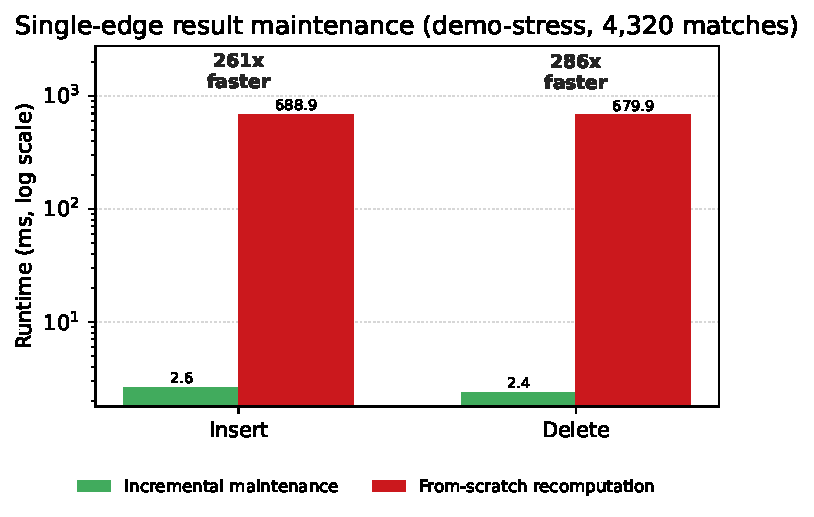
\includegraphics[width=0.6\linewidth]{figures/dynamic_speedup.pdf}
  \caption{Incremental single-edge maintenance vs.\ from-scratch recomputation on the demo-stress graph (log scale). Maintenance cost is governed by the small affected set, not the full result size, giving a two-orders-of-magnitude speedup. Source: \texttt{reports/figures/plot\_dynamic.py} (data \texttt{dynamic\_data.csv}).}
  \label{fig:dynamic}
\end{figure}

The results support three observations. First, correctness holds in every case: the incrementally maintained result set, including the precise added and removed mappings, matches the from-scratch recomputation. Second, the benefit is governed by locality. On the toy graph the incremental method is actually marginally \emph{slower}, because its fixed setup cost (candidate construction and anchor enumeration) dominates when the whole graph has only two matches; this marks the small-input overhead floor. Third, once the result set is non-trivial the advantage becomes decisive (Figure~\ref{fig:dynamic}): on the demo-stress graph the incremental method explores only $6$ partial mappings and finishes in about $2.5$\,ms, whereas recomputing the full result set (all $4{,}320$ mappings) takes roughly $0.68$--$0.69$\,s, a speedup of more than two orders of magnitude. This matches the locality property: the cost of maintenance scales with the size of the affected set $D_e$, not with the size of the full result.

The same harness accepts the real \texttt{.graph} workloads used in the main experiments via \texttt{-{-}input-format graph}, so the table can be extended to Yeast, Human, and HPRD once those datasets are placed under \texttt{data/raw/}. This extension only supports single-edge updates on a fixed query; batched updates, vertex insertion and deletion, and reuse of the recorded partial-mapping structure across successive updates are left as future work. Even in this restricted setting, the experiments show that single-edge result maintenance can be made effectively independent of the total result size.
